
%(BEGIN_QUESTION)
% Copyright 2011, Tony R. Kuphaldt, released under the Creative Commons Attribution License (v 1.0)
% This means you may do almost anything with this work of mine, so long as you give me proper credit

To ulike nivåtransmittere brukes som redundant måling for en kritisk tank i en petrokjemisk raffineringsprosess der høyt nivå er farlig, men lavt nivå er sikkert.  En ``high select''-avstemmingsalgoritme ignorerer det laveste transmittersignalet.  Pålitelighetsverdien ($R$) for hver transmitter -- sannsynligheten for å måle væskenivået korrekt i tanken -- er vist i diagrammet:

$$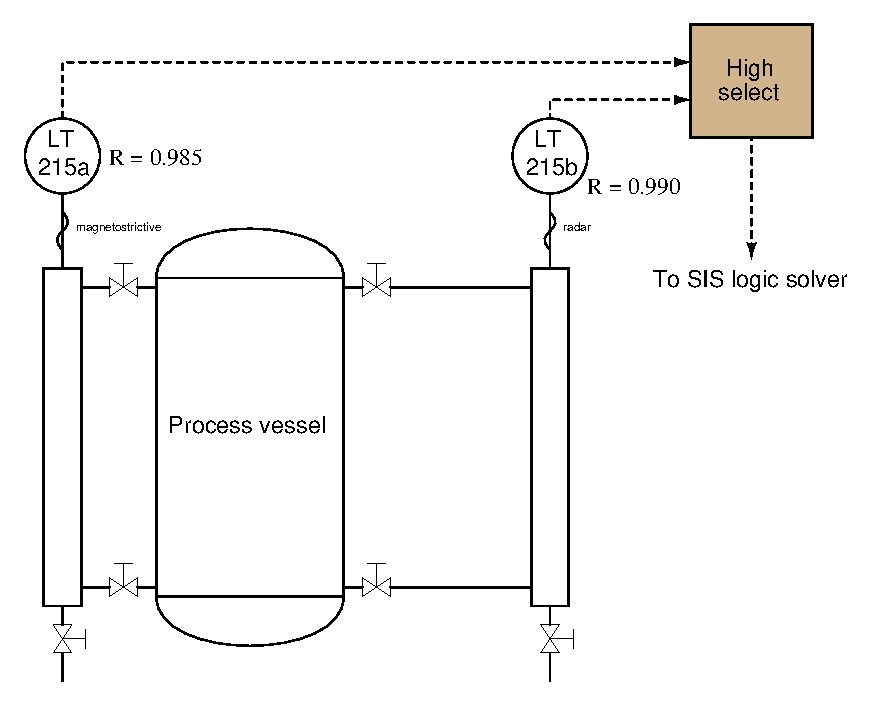
\includegraphics[width=15.5cm]{i00225x01.eps}$$

Bestem {\it MooN}-klassifiseringene for dette redundante transmittersystemet, både fra perspektivet {\it dependability} (dvs. {\it MooN}-klassifiseringen som beskriver evnen til å oppdage en farlig (høy) nivåtilstand), og fra perspektivet {\it security} (dvs. {\it MooN}-klassifiseringen som beskriver evnen til å holde prosessen i gang).

\vskip 10pt

MooN (dependability) = \underbar{\hskip 50pt}  \hskip 70pt MooN (security) = \underbar{\hskip 50pt}

\vskip 40pt

Beregn deretter total pålitelighet for at dette to-transmittersystemet vil kunne initiere en nedstengning ved behov, basert på de oppgitte individuelle pålitelighetsverdiene:

\vskip 10pt

$R_{shutoff}$ = \underbar{\hskip 50pt}

\underbar{file i00225}
%(END_QUESTION)





%(BEGIN_ANSWER)

{\it 2 poeng for hvert MooN-svar, pluss 6 poeng for pålitelighetsberegningen}

\vskip 10pt

MooN (dependability) = \underbar{\bf 1oo2}  \hskip 70pt MooN (security) = \underbar{\bf 2oo2}

\vskip 10pt

$R_{shutoff}$ = \underbar{\bf 0.99985}

%(END_ANSWER)





%(BEGIN_NOTES)

{\bf Dette spørsmålet er ment for eksamen og ikke arbeidsark!}

%(END_NOTES)
